\documentclass[a4paper,10pt]{report}
\usepackage[utf8x]{inputenc}
\usepackage[english,russian]{babel} 
\usepackage{graphicx}

\usepackage{amssymb}
\usepackage[12pt]{extsizes}
\usepackage{epigraph}
\usepackage{fixme}
\usepackage{rotating}
\usepackage{amsmath}
\usepackage{hyperref}

\usepackage[12pt]{extsizes}
\usepackage[left=3cm,right=2cm,top=2cm,bottom=2cm]{geometry}
\renewcommand{\baselinestretch}{1.5}

% Title Page
\title{Разработка алгоритмов обеспечения качества распределенного поисковго робота для сети Интернет}
\author{Волков Сергей}



\begin{document}
\begin{titlepage}
\begin{center}

\textsc{САНКТ-ПЕТЕРБУРГСКИЙ ГОСУДАРСТВЕННЫЙ УНИВЕРСИТЕТ}\\
\textsc{Математико-механический факультет}\\[1.0cm]

\textsc{Кафедра системного программирования}\\[3.0cm]

{ \LARGE Разработка алгоритмов обеспечения качества}\\[1.0cm]
{ \LARGE распределенного поискового робота}\\[1.0cm]
{ \LARGE для сети интернет}\\[1.0cm]
{Дипломная работа студента 545 группы \\ Волкова Сергея Андреевича}\\[3.0cm]

\begin{tabular}{lcr}
Научный руководитель & ……………… & ассистент кафедры АСОИУ СПбГЭТУ ЛЭТИ\\ & & Выговский Л.С \\
& /подпись/ & \\[1.0cm]
Рецензент            & ……………… & ст.преп. Луцив Д.В \\
& /подпись/ & \\[1.0cm]
``Допустить к защите'' & ……………… & д.ф.-м.н., проф. Терехов А.Н. \\
заведующий кафедрой, & /подпись/ & \\
\end{tabular}

\vfill

{\large Санкт-Петербург \\ 2011}

\end{center}
\end{titlepage}

\begin{titlepage}
\begin{center}
\begin{otherlanguage}{english}

\textsc{SAINT PETERSBURG STATE UNIVERSITY}\\
\textsc{Mathematics \& Mechanics Faculty}\\[1.0cm]

\textsc{Software Engineering}\\[3.0cm]

{ \LARGE Development of quality assurance algorithms}\\[1.0cm]

{ \LARGE for the distributed web crawler}\\[1.0cm]

{by \\ Sergey Volkov \\ Master’s thesis}\\[3.0cm]

\begin{tabular}{lcr}
Supervisor & ……………… & L.S Vygovsky \\[1.0cm]
Reviewer            & ……………… & Senior Lect. D.V Luciv\\[1.0cm]
``Approved by'' & ……………… & Professor A. N. Terekhov\\
Head of Department, & & \\
\end{tabular}

\vfill

{\large Saint Petersburg \\ 2011}

\end{otherlanguage}
\end{center}
\end{titlepage}

\maketitle
\tableofcontents

% \makeindex
% \begin{abstract}
% \end{abstract}

\chapter{Введение}
\section*{Цель}
Целью данной работы является оптимизация процесса сборки документов системой nutch.
\section*{Nutch}
Nutch - свободное программное обеспечение для интернет поиска.
Nutch основан на поисковом движке Lucene\cite{lucene}, с набором средств для работы с web, таких как поисковый робот, база ссылок, парсеры для html и других форматов и.т.п.
Nutch работает поверх фреймворка hadoop.
\section*{Hadoop}
\label{sec:hadoop}
Hadoop является свободным Java фреймворком, поддерживающим выполнение распределённых приложений, работающих на больших кластерах, построенных на обычном оборудовании. Hadoop прозрачно предоставляет приложениям надёжность и быстродействие операций с данными. В Hadoop реализована вычислительная парадигма, известная как MapReduce.
\section*{MapReduce}
\label{sec:mapred}
Общая идея MapReduce состоит в том, чтобы представить алгоритм в виде набора последовательных этапов, из которых каждый состоит из двух шагов - map и reduce (возможны дополнительные шаги - combine и partition). Система разбивает входные данные на пары $\langle key, value\rangle$, над каждой парой выполняется функция map на выходе которой, должен получится набор пар $\langle key, value\rangle$. 
Сгенерированные данные система реорганизует и для каждого из них выбирает узел на котором исполнится процедура reduce. Данные для одного reduce узла группируются по одинаковым ключам и ключи сортируются. После чего данные, в виде $\langle key, value*\rangle$ опять передаются пользователю, который производит над ними операцию reduce (свёртка) на каждом узле. Получившиеся на выходе пары $\langle key, value\rangle$ передаются в выходной поток (Рис.~\ref{ris:mapreduce}).
  \begin{figure}[h]
    \center{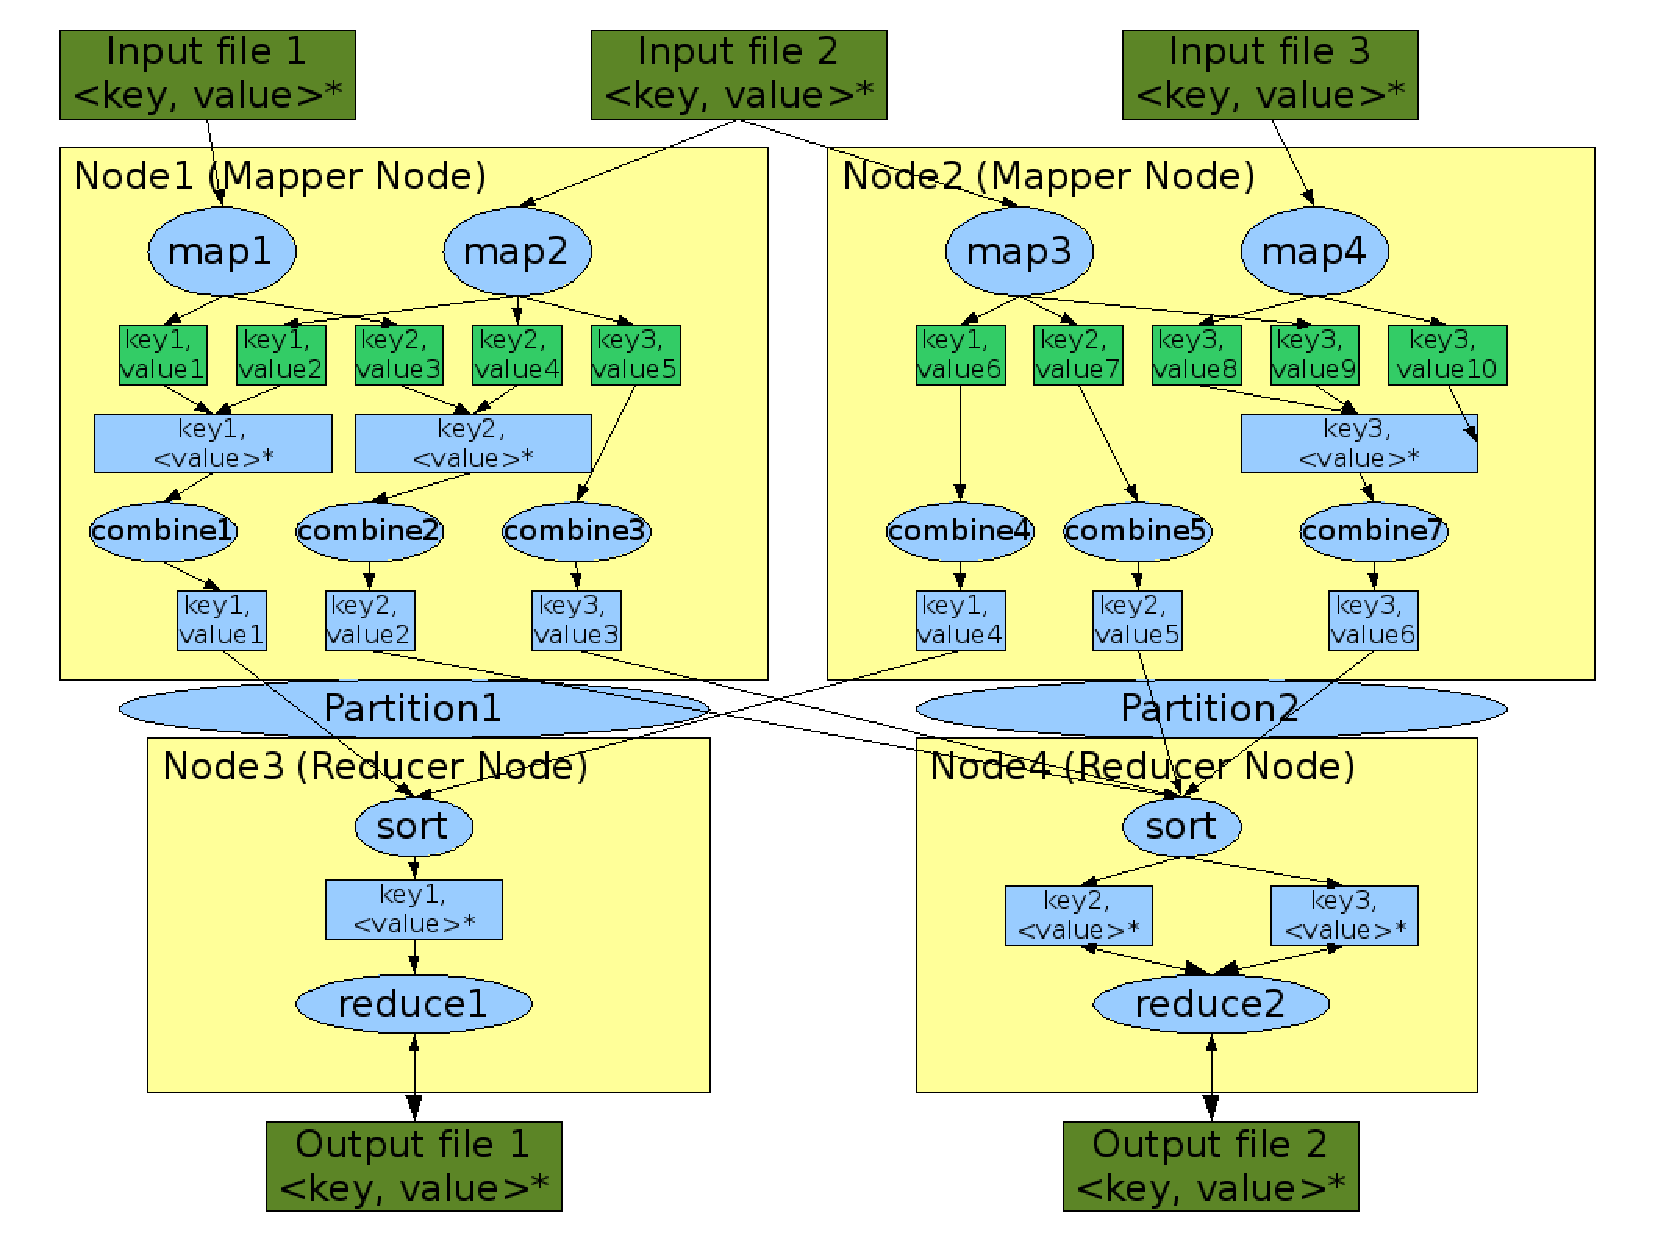
\includegraphics[width=1\linewidth]{img/mapreduce}}
    \caption{Схема MapReduce\cite{pimenov} }
    \label{ris:mapreduce}
  \end{figure}

Преимущество MapReduce заключается в том, что он позволяет распределенно производить операции предварительной обработки и свертки. Операции предварительной обработки работают независимо друг от друга и могут производиться параллельно. Аналогично, множество рабочих узлов могут осуществлять свертку — для этого необходимо только чтобы все результаты предварительной обработки с одним конкретным значением ключа обрабатывались одним рабочим узлом в один момент времени. Таким образом MapReduce может быть применен к большим объемам данных, которые могут обрабатываться большим количеством серверов.\cite{hadoop}
\section*{Работа nutch с точки зрения MapReduce}
Сборка осуществляется итеративно - на каждой итерации осуществляется выбор url для загрузки, загрузка, индексация полученных данных, обновление базы ссылок и обновление базы обратных ссылок. 
  \begin{figure}[h]
    \center{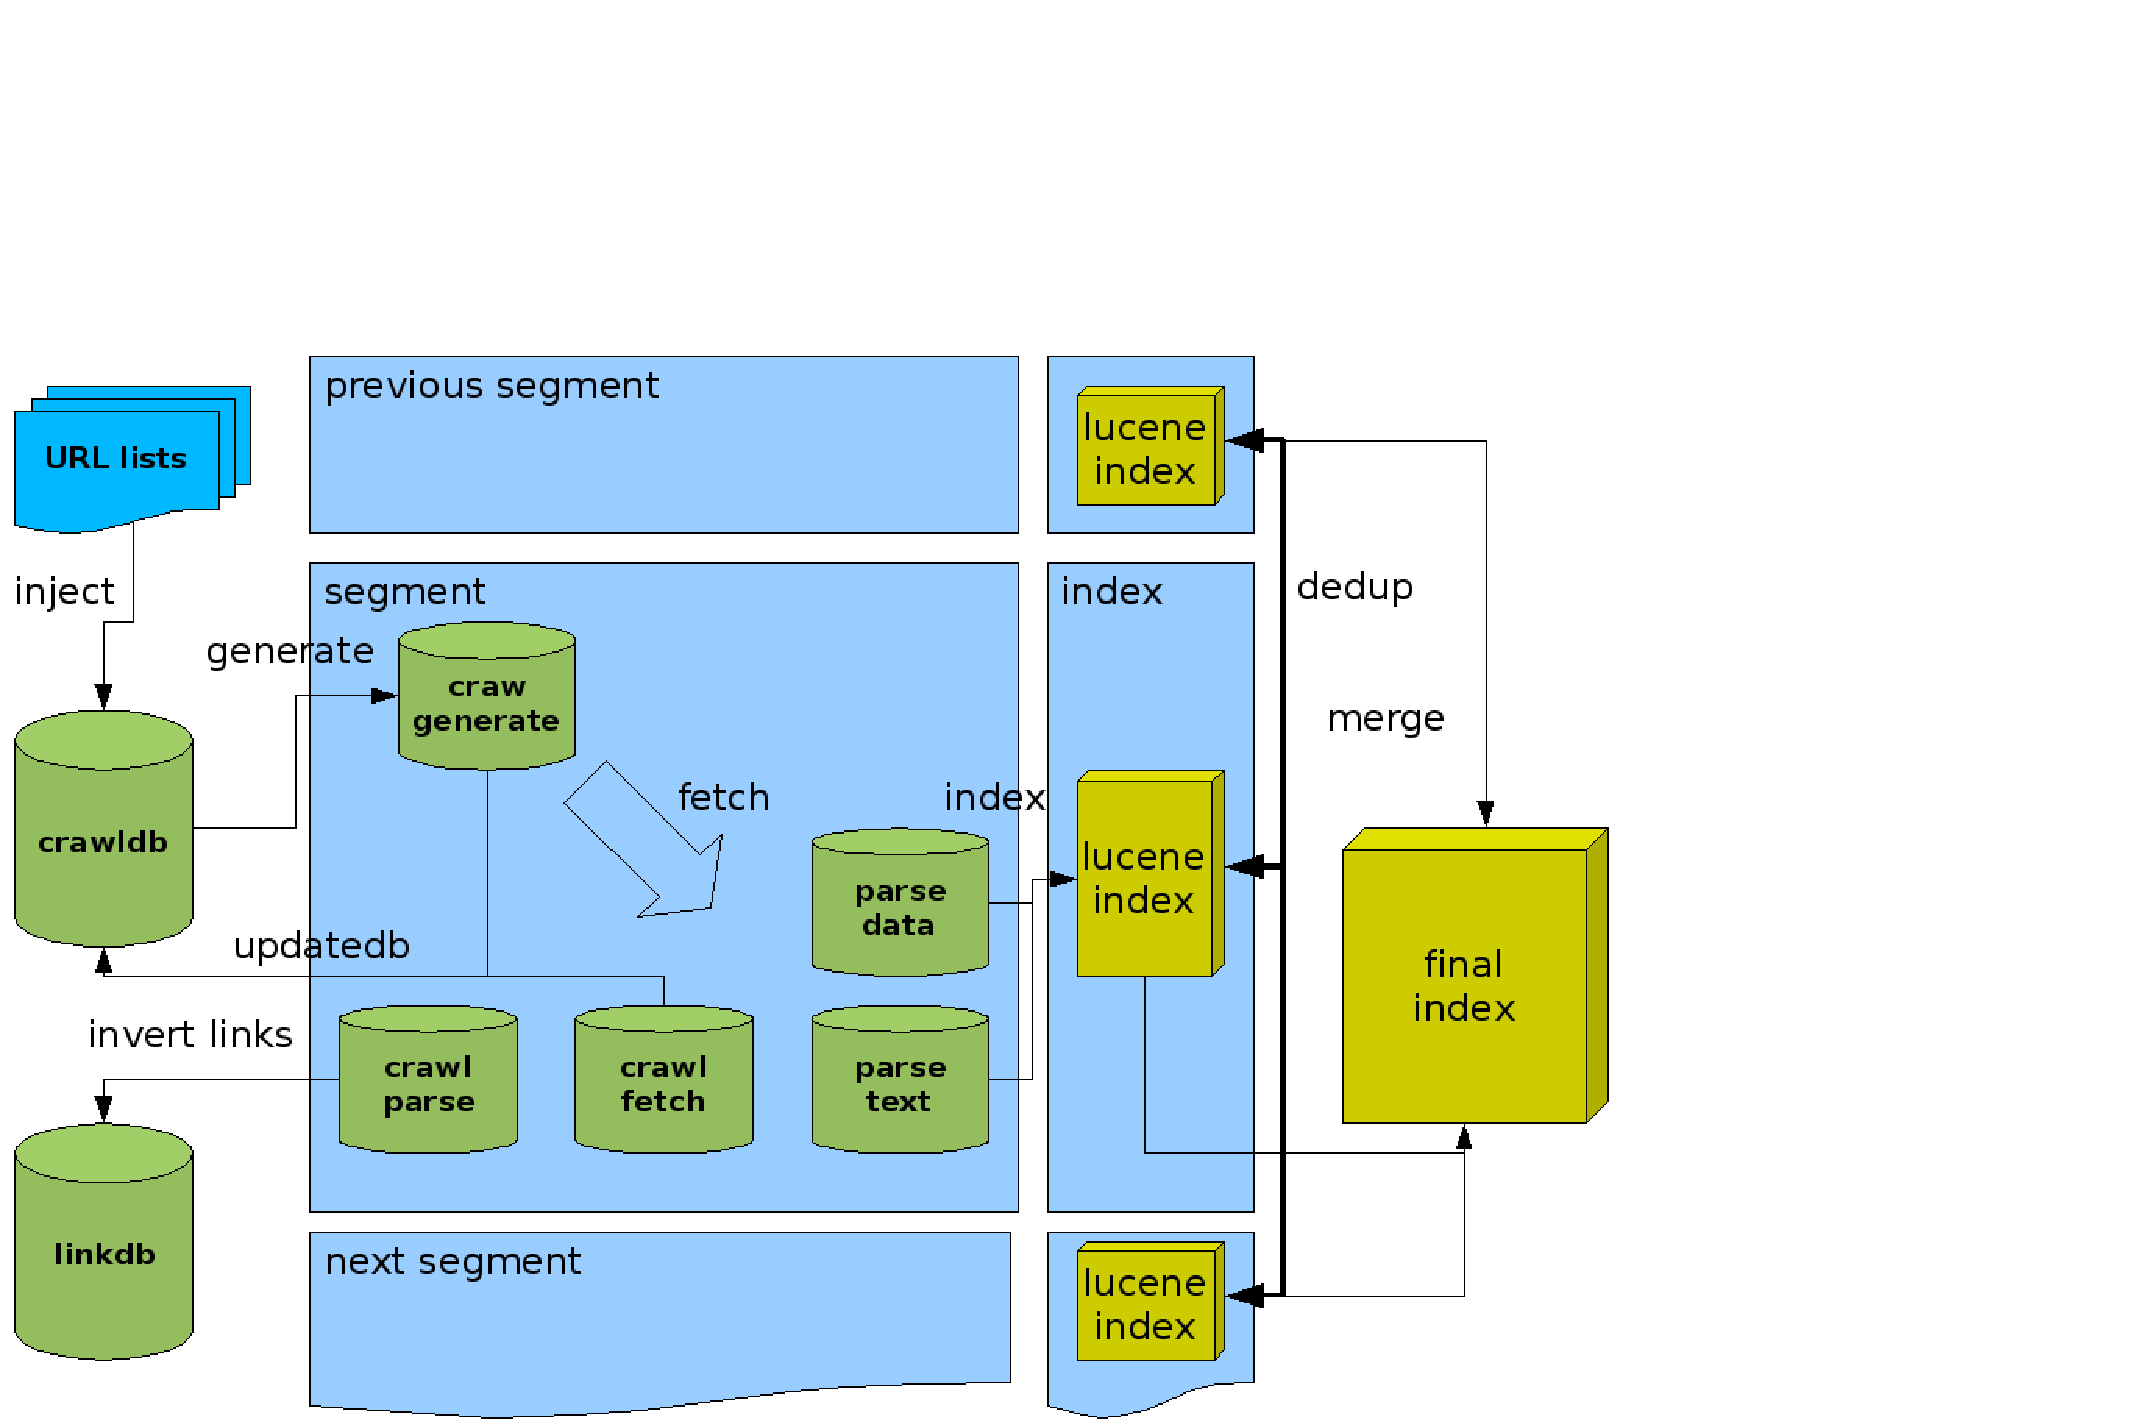
\includegraphics[width=1\linewidth]{img/nutch}}
    \caption{Работа Nutch\cite{pimenov}}
    \label{ris:nutch}
  \end{figure}

На рис. ~\ref{ris:nutch} представлена схема работы nutch, при этом приняты следующие обозначения: 
\begin{itemize}
 \item \texttt{generate} --- выбор url из общей базы (crawldb)
 \item \texttt{fetch} --- загрузка документов по url
 \item \texttt{index} --- создание индекса по скачанным документам
 \item \texttt{merge} --- слияние индекса по сегменту с основным
 \item \texttt{dedup} --- удаление дубликатов из индекса
 \item \texttt{updatedb} --- обновление crawldb
 \item \texttt{invert links} --- создание и обновление базы обратных ссылок (linkdb)

\end{itemize}


\section*{Условия}
Задача web сборки заключается в нахождении нужных url и скачивания документов по ним, большинство url появляется из уже скачанных документов.
Иногда непосредственно по url можно определить что документ является ``полезным''. Например, для того, что бы скачать все новости с ресурса lenta.ru, достаточно скачивать документы по url который можно задать регулярным выражением \ref{eq:lentaregex}

\begin{equation} \label{eq:lentaregex}
http://lenta\textbackslash.ru/news/\textbackslash d\{4\}/\textbackslash d\{2\}/\textbackslash d\{2\}/\textbackslash w+/
\end{equation}
 
\section*{Постановка задачи}
Необходимо изменить nutch для работы с учетом информации о ``полезности'' ссылок.

Основные требования:
\begin{itemize}
 \item минимальные изменения ядра nutch
 \item возможность обновления информации о ссылках без остановки сборки
 \item возможность работы без вмешательства администратора
\end{itemize}
\section*{Актуальность}
Nutch является активно развивающимся проектом, на его основе сейчас создан один из крупнейших поисковиков по исходному коду \href{http://www.krugle.com/}{Krugle}. Одна из основных проблем web-поиска это чрезмерное количество данных. Скачать все даже с одного ресурса крайне ресурсоемкая задача, и даже не всегда выполнимая - т.к. как многие документы создаются динамически, и возможно ``зацикливание''. 

Не смотря на то, что практически каждый ресурс содержит информацию по сборке (robots.txt), не редко огромное количество совершенно бесполезных ссылок и дубликатов не попадает под фильтры, отсюда вытекает необходимость контроля хода сборки в соответствии с дополнительной информацией о url.

\chapter{Алгоритмы}
Поскольку WWW представляет собой крайне сложную среду, которая постоянно развивается, предпочтение было отдано практическому подходу:
\begin{enumerate}
 \item запустить систему без модификаций;
 \item найти самое слабое место в системе;
 \item принять меры по его устранению;
 \item перейти к пункту \textit{2}.
\end{enumerate}

Данный процесс завершается в момент, когда становится понятно, что система сможет выдерживать необходимую нагрузку на достаточном промежутке времени, и дальнейшие улучшения неоправданны.
\section{Ранжирование}
При работе системы в стандартной конфигурации было замечено, что только из 10\% скачиваемых веб-страниц выделяются документы. Это происходит из-за не оптимального упорядочивания ссылок из \textit{сrawldb}.

Определение порядка выбора URL для скачивания существенно сказывается на эффективности работы робота.\cite{crawl}\cite{focused}\cite{opic} Порядок неважен только в том случае, если робот нацелен на одноразовое скачивание всего Web, и нагрузка создаваемая роботом на целевые сайты не важна, так как тогда каждая известная URL будет в конце концов загружена. Однако, большинство роботов не способно посетить каждый URL по трем основным причинам.
\begin{itemize}
 \item Ограничение по ресурсам --- размер хранилища, ширина канала, CPU time для обработки страниц.
 \item Сбор документов занимает время, поэтому в определенный момент робот вынужден заново посещать некоторые страницы для нахождения изменений.
 \item Динамическое создание страниц --- сейчас большинство сайтов раздают не статический контент, а создают его динамически при помощи скриптов обрабатывающих URL и возвращающих результат, таким образом количество страниц на сайте может быть неограниченно.
\end{itemize}

Во всех остальных случаях существенно что бы робот сначала посещал ``важные'' страницы. Ранжирование отвечает за определение того, на сколько URL ``важна''.
В Nutch порядок выбора URL определяется в плагинах подключенных к точке расширения \textit{ScoringFilter}, в результате работы которых каждой URL сопоставляется \textit{score}. На каждой итерации для скачивания выбираются URL с наибольшим score.

В стандартной конфигурации Nutch для выбора ссылок используется \textit{OPIC Score} плагин.
\subsection{OPIC}
\textit{OPIC} --- On-Line Page Importance Computation\cite{opic}. Данный алгоритм рассчитывает важность страницы на основе важности страниц на него ссылающихся. В отличии от off-line методов, когда сначала скачивается часть Web, а потом на основе полученного графа ссылок вычисляется важность страниц, этот метод позволяет работать когда большая часть сетевого графа еще не известна.

В Nutch реализована упрощенная версия данного алгоритма, при котором в момент скачивания страницы к score каждой из ссылок с нее (\textit{outlink}) добавляется $S_{0}/n$ где $S_{0}$ --- $score$ скачанной страницы, а $n$ --- число исходящих ссылок. Данный способ плохо подходит для поиска новостей, поскольку для новостей основным признаком ``важности'' веб-страницы является присутствие в нем текста новости, что на практике не связано с количеством входящих ссылок.

Поскольку в системе идентификация новостей производится только по URL, возникает желание скачивать только те URL, которые подходят под правила.

\subsection{Предложенный алгоритм}
Так как в Nutch можно использовать одновременно сразу несколько ScoringFilter'ов (полученные из различных алгоритмов \textit{score} просто перемножаются), вместо изменения стандартного метода следует создать отдельный плагин, который всем новым поступающим в систему URL, подходящим под правила разбора, устанавливал $score=s_{fit}$ и $s_{n}$ остальным.
\subsection{Особенности реализации}
Данная функциональность была реализована при помощи двух плагинов. Первый проверяет является ли URL ``полезной'', и добавляет необходимую информацию в $crawldatum$ (в \textit{crawldb} хранятся записи вида $\langle URL, crawldatum\rangle$, где \textit{crawldatum} --- различная дополнительная информация об URL), а второй выставляет ранг согласно $crawldatum$ и настроек приложения. Такое разбиение было сделано потому, что информация о том, что URL является ``полезной'', представляет собой интерес и без использования данного ранжирования (например, это было использовано при получении статистики).
\subsubsection*{SkaiScoringMeta}
\label{sec:scoringmeta}
SkaiScoringMeta --- плагин, являющийся расширением к точке ScoringFilter, выделяющий ``полезные'' URL. Для хранения дополнительной информации в $crawldatum$ используется поле $metaData$, которое представляет собой набор пар вида $\langle key, value\rangle$
Для сохранения индикатора ``полезности'' в мета данные $crawldatum$ добавляется пара $\langle skai.scoring.fit, true\rangle$.

Для определения ``полезности'' URL используется кэш с регулярными выражениями, загружаемыми из базы данных при инициализации. Поскольку таких регулярных выражений может быть много (хотя бы по одному на сайт) и они разбиты по доменам, для сокращения времени проверки каждой URL используется хэш вида $\langle domainname, regex^{+}\rangle$, таким образом время проверки URL практически не зависит от числа доменов.

Так же, для уменьшения числа проверок, метаданные добавляются не в момент первого обнаружения ссылки системой (сразу после разбора веб-страницы), а только в момент добавления уникальной URL в \textit{crawldb}, что уменьшает число проверок приблизительно в 10 раз, так как в среднем только 9\% исходящих со страницы ссылок не были ранее известны.
\subsubsection*{SkaiScoring}
SkaiScoring --- плагин являющийся расширением к точке ScoringFilter, выставляющий $score$. Для ссылок только что попавших в систему, зависимости от наличия мета тега, выставляет значения $score$ либо $s_{fit}$, либо $s_{n}$, где коэффициенты $s_{fit}$ и $s_{n}$ получаются из файла конфигурации Nutch.
\subsection{Результат}
При использовании стандартных ScoringFilter'ов в среднем за цикл, из всех скачиваемых ссылок ``полезных'' скачивалось порядка 10\% (В качестве пространства поиска использовалось 40 крупнейших СМИ, на каждой итерации выбиралось 20000 ссылок, ``полезными'' признавались непосредственно новости). А при использовании данных плагинов уже на ранней стадии сборки порядка 80\% ссылок были ``полезными'' (Рис.~\ref{ris:score}). Благодаря предложенным оптимизациям время цикла практически не изменилось по сравнению с временем работы в стандартной конфигурации. Таким образом было получено увеличение эффективности в восемь раз по сравнению с базовой реализацией Nutch.

\begin{figure}[h!]
 \center{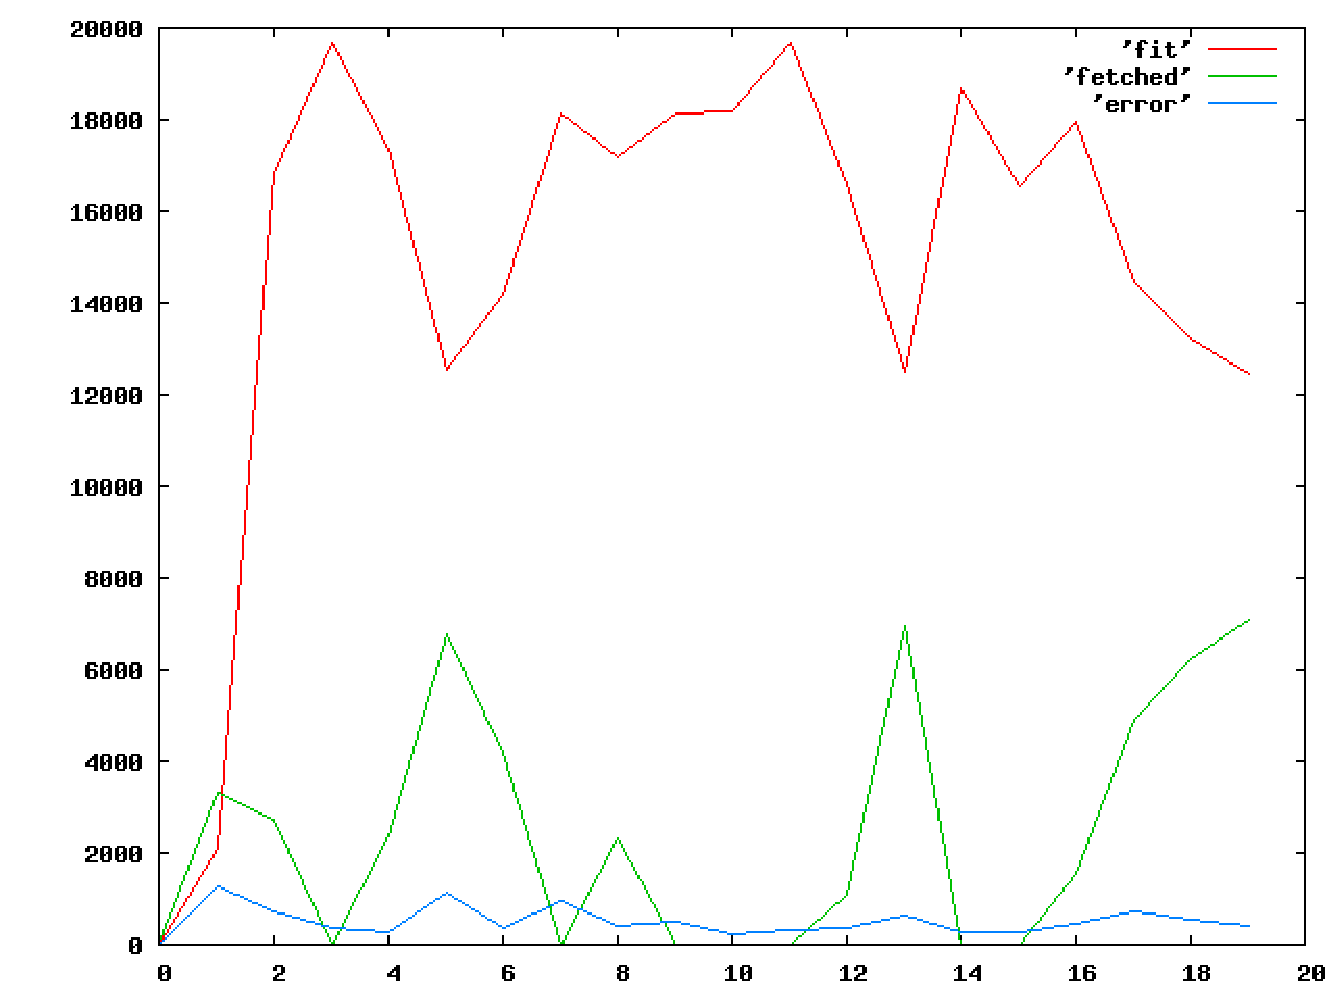
\includegraphics[width=0.8\linewidth]{img/scoring}}
 \caption{График зависимости числа ссылок от номера итерации. fit---число полезных ссылок, fetched---число скачанных ссылок не являющихся полезными, error---число ошибок при скачивании}
 \label{ris:score}
\end{figure}

\section{Работа Nutch с индексом}
Время используемое для слияния полученного из сегмента индекса с основным растет пропорционально размеру индекса. Этот этап не работает через MapReduce и фактически выполняется на одной машине, что приводит к простою кластера. Для индекса содержащего 2 миллиона документов (70GB) только копирование индекса из HDFS в локальную файловую систему и обратно занимает больше двух часов (при скорости локальной сети 20Mb/s), а общее время работы достигает 11 часов ($2\times2,5$ GHz 2007 Xeon, 1,7GB RAM, скорость последовательного доступа к диску 50MB/s). При размере \textit{crawldb} в 80 миллионов ссылок и генерации сегмента в 80 тысяч URL на слияние индюка уходит 68\% от общего времени цикла (на кластере из трех узлов).
\subsection{Lucene}
\textit{Lucene} --- библиотека полнотекстового поиска. Индекс Lucene построен по принципу обратного файла (инвертированного индекса). Сам индекс состоит из сегментов, каждый из которых грубо говоря представляет отсортированный список термов. Для ускорения поиска сегменты ``склеиваются'' в один. Операция ``склеивания'' представляет собой этап слияния из сортировки слиянием, и производится за время прямо пропорциональное сумме размеров склеиваемых сегментов. По умолчанию Nutch хранит индекс в одном сегменте, к которому на каждой итерации ``приклеиваются'' новые сегменты индекса, таким образом за каждую итерацию весь индекс перезаписывается.

Было рассмотрено несколько подходов к решению данной проблемы:
\begin{itemize}
 \item \textbf{Асинхронное обновление} --- выделяется отдельный поток, который  находит все новые сегменты, скачивает их и независимо от процесса основной сборки и обновляет индекс. При этом время на слияние индексов не влияет на скорость скачивания документов, однако, уже при размере индекса в 5,3 миллионов документов индекс будет обновляться только один раз за сутки, из-за чего новости за последние 30 часов никогда не появятся в индексе (время на слияние+время цикла).
 \item \textbf{Изменение политики слияния} --- хранение индекса в одном сегменте требует перезаписи всего индекса при каждом обновлении. При этом если вообще не ``склеивать'' сегменты, существенно падает время поиска в индексе, поскольку приходится искать терм в большом числе словарей. Необходимо разработать алгоритм который позволял бы контролировать число сегментов, при этом не перезаписывая основную часть индекса.

Приблизительно, время выполнения запроса можно оценить следующим образом: $t_{q} = \sum\limits_{s\in S} td_{s} + ti$, где $td_{s}$ это поиск термов в словаре сегмента $s$, а $ti$ --- время на пересечение списков документов соответствующих термам. Причем $ti$ прямо пропорционально количеству документов соответствующих термам, а $td_{s} = O(\log n_{s})$, где $n_{s}$ --- размер словаря сегмента, который практически не зависит от размера сегмента, и можно считать константой. Само время ``склеивания'' сегментов прямо пропорционально их размеру, из чего следует что эффективнее всего склеивать между собой самые маленькие сегменты. 
 
\end{itemize}
\subsection{Алгоритмы}
\subsubsection{Асинхронное обновление}
Поскольку появление новых сегментов происходит один раз за несколько часов, было решено создать процесс, который через определенные промежутки времени проверяет наличие новых сегментов и скачивает их стандартными средствами Hadoop в локальную файловую систему клиента работающего с индексом, после чего сообщает клиенту о необходимости подключить новые сегменты.
\subsubsection{Политика слияния}
Индексам присваивается некий уровень $l$, так же известно максимальное количество сегментов на каждом уровне $N_{l}$. Всем только что скачанным сегментам присваивается $l=0$, в тот момент когда количество индексов на каком-то из уровней превышает $N_{l}$ они ``склеиваются'' в один сегмент уровня $l+1$.
\subsection{Особенности реализации}
\subsubsection{Асинхронное обновление}
Как только заканчивается индексация нового сегмента, к имени сегмента добавляется префикс \textit{ready}. Процесс просматривает папку с сегментами в HDFS и при наличии сегментов с такими префиксами скачивает их и убирает префикс, после чего сообщает клиенту HTTP запросом о необходимости подключить новый сегмент. При таком подходе аварийное завершение процесса обновления не влечет никаких последствий --- достаточно просто заново его запустить, и отключение основного цикла сборки никак не сказывается на процесс обновления (кроме того, что не появляется новых сегментов индекса).
\subsubsection{Политика слияния}
Индексы были разбиты на следующие уровни:
\begin{enumerate}
 \item new --- новые сегменты;
 \item daily --- сегменты за день;
 \item weeky --- сегменты за неделю;
 \item monthly --- сегменты за 4 недели;
 \item 1-level --- сегменты за 4 месяца ($4\times4$ недели);
 \item k-level --- сегменты получаемые при слиянии четырех k-1-level.
\end{enumerate}
В конце каждого дня все новые индексы объединяются в дневные, как только их набирается 7 --- они склеиваются в недельные и.т.д. Сама функциональность была реализована как \textit{Groovy} скрипт.
\subsection{Результат}
Благодаря асинхронному обновлению время цикла уменьшилось на 68\%, однако возросла нагрузка на сервер осуществляющим поиск, так как слияние индексов стало происходить на нем, однако, за счет новой политики слияния, каждый документ в индексе перезаписывается не более 5 раз за год, что дает в сумме не более 80 часов в год при конечном индексе в 10 миллионов документов.
 

\section{Раннее удаление дубликатов}
Для выдачи качественных результатов поиска важно что бы в индексе не было дубликаов. Под дубликатом понимаются:
\begin{itemize}
 \item web-страницы с одинаковым URL;
 \item web-страницы с одинаковым текстом и доменом. 
\end{itemize}
\subsection{Реализация в Nutch}
В Nutch удаление дубликатов реализовано в виде серии MapReduce задач и работает достаточно быстро --- на дедубликацию как правило уходит не больше 3\% от общего времени. Однако у этого метода есть ряд существенных недостатков.
\begin{itemize}
 \item Дедубликация происходит уже после индексации документов. При этом дубликаты тоже индексируются, что занимает существенно большее время (порядка 10\% от общего времени цикла).
 \item Для эффективной работы MapReduce желательно что бы индекс хранился в распределенной файловой системе, а для быстрого поиска по индексу необходимо наличие копии в локальной файловой системе. Таким образом  нужно постоянно хранить согласованные копии индекса в двух файловых системах.
 \item Для удаления дубликатов достаточно знать только набор md5 хэшей и URL, а приходится читать весь индекс.
\end{itemize}
\subsection{Алгоритм}
Поскольку для удаления дубликатов достаточно небольшого количества данных (URL + md5 для каждого документа) было решено использовать Key Value базу данных. После получения текста статьи проверяется есть ли в базе данных такой хэш или URL, если есть, то страница отбрасывается, иначе в базу добавляются данные о новой странице и страница индексируется. Основным недостатком данного подхода является невозможность обновления документа (так как мы не изменяем уже готовые части индекса). В рамках данной системы это не критично, так как интересует появление новых новостей, а не обновление старых.

Поскольку сервер с базой данных должен справляться с нагрузкой с целого кластера был произведен анализ различных реализаций Key Value СУБД.
\subsection{Сравнение Key Value СУБД}
Были рассмотрены следующие реализации:
\begin{itemize}
 \item Memcached\footnote{\href{http://memcached.org/}{http://memcached.org/}} --- система кэширования данных разработанная для ускорения веб приложений. Изначально была создана для LiveJournal в 2003 году. Данные хранятся только в памяти, что позволяет осуществлять быстрый доступ, но при этом необходимо отдельно заботиться о сохранении данных на диск.
 \item MongoDB\footnote{\href{http://mongodb.org/}{http://mongodb.org/}} --- документо-ориентированная Key Value СУБД. MondoDB позиционирует себя как промежуточное звено между простейшими Key Value хранилищами и реляционными СУБД.
 \item Project Voldemort\footnote{\href{http://project-voldemort.com/}{http://project-voldemort.com/}} --- распределенное отказоустойчивое Key Value хранилище. Одним из приемуществ данной системы является отсутсвие единой точки отказа (single point of failure). Project Voldemort используется в качестве хранилища данных в LinkedIn\footnote{\href{http://www.linkedin.com/}{http://www.linkedin.com/}}.
 \item Tokyo Cabinet\footnote{\href{http://fallabs.com/tokyocabinet/}{http://fallabs.com/tokyocabinet/}} --- встроенное Key Value хранилище. Поддерживает как хранение данных только в памяти, так и на диске. Для удаленного доступа используется Tokyo Tyrant\footnote{\href{http://fallabs.com/tokyotyrant/}{http://fallabs.com/tokyotyrant/}}. Протокол Tokyo Tyrant почти полностью совместим с Memcached.
\end{itemize}

Сравнение данных СУБД представлено в таблице \ref{tab:kv}.

\begin{table}[h]
\caption{\label{tab:kv}Сравнение Key Value СУБД.}
\begin{center}
\begin{tabular}{|c|c|c|c|c|c|c|}
\hline
Название & Memcached & MongoDb & Project Voldemort & Tokyo Cabinet\\
\hline
Операции put/ms & 4.03 & 6.65 & 1.21 & 3.25 \\
\hline
Операции get/ms & 4.54 & 3.05 & 1.01 & 4.39 \\
\hline
Устойчивость & - & + & + & + \\
\hline
Распределенность & + & + & + & - \\
\hline
Репликация & - & + & + & - \\
\hline
Модель данных & bin & object & object & bin\\
\hline
\end{tabular}
\end{center}
\end{table}

\subsubsection{Измерение производительности}
Так как время выполнения put и get запросов является критическим для нашей системы, было решено разработать утилиту\footnote{\href{http://github.com/volkov/kvstorage-test}{http://github.com/volkov/kvstorage-test}} измеряющую производительность различных СУБД на данных, с которыми потом будет осуществляться работа. Результаты данных тестов представлены в строчках put и get таблицы \ref{tab:kv}.

Тестирование происходило по следующему сценарию:
\begin{enumerate}
 \item в базу добавляются все URL из рабочего индекса (5688210 ссылок);
 \item проверяется наличие всех URL из индекса по одному из сегметнов (52583 ссылок).
\end{enumerate}
Добавление и проверка производятся в 10 потоков. Сервер и клиент находятся на разных хостах ($1.2$ GHz 2007 Xeon, 1.7GB RAM, скорость последовательного доступа к диску 50MB/s), время ping между хостами --- 0.6ms.
\subsubsection{MongoDB}
В качестве Key Value СУБД была выбрана MongoDB так как она проста в настройке, достаточно надежна и производительна. MongoDB поддерживает несколько \textit{баз данных} на одном сервере (аналог \textit{database} в реляционных СУБД), а так же различные \textit{коллекции} (аналог таблиц) внутри одной базы данных. Из недостатков можно отметить отсутвие какой-либо авторизации и аутентификации, но поскольку кластер работает в DMZ это не существенно.                                                                                                                                                                                                                                                                                        
\section{Особенности реализации}
Данная функциональность была реализована как плагин с точкой расширения \textit{IndexingFilter}. Плагины этой точки расширения, как правило, применяются для добавления полей к индексируемому документу, но так же подходят и для отсечения ненужных документов.

Данные в MongoDB хрянятся в коллекциях \textit{url} и \textit{hash}, в которых хранятся записи вида $\langle url,segmentid,taskid \rangle$ и $\langle md5,segmentid,taskid \rangle$ соответственно.
\textit{Segmentid} и \textit{Taskid} хранятся для того, что бы определить ситуацию когда Hadoop по различным причинам перезапустил часть задачи (это просиходит при некорректном завершении частей задач, или когда определенная часть задачи выполняется слишком медленно). В таком случае, несмотря на наличие записи в MongoDB, фильтр пропускает документ. Фильтр работает следующим образом:
\begin{enumerate}
 \item если в MongoDB нет ни записи с соответствующим $url$, ни записи с соответствующим $md5$, они добавляются и документ пропускается;
 \item если в MongoDB есть запись с данным $url$ и $md5$, и $taskid$ в них совпадает с текущей, документ пропускается;
 \item во всех остальных случаях документ фильтруется.  
\end{enumerate}

В случае некорректного завершения всей задачи, все записи с текущим $segmentid$ удаляются.

\section{Результаты}
Время на проверку документа в базе данных практически не сказалось на времени индексации, поскольку индексация в основном загружает процессор и производится в несколько потоков. Так что во время ожидания ответа от MongoDB обсчитывается другой документ. При этом необходим дополнительный сервер с базой данных, который может быть объединен с сервером осуществляющим поиск или любым другим.

Время которое экономится за счет того, что дубликаты не индексируются, напрямую зависит от количества дубликатов в выборке. При использовании системы в реальных условиях данных подход позволяет экономить до 44\% на этапе индексации.

Поскольку операция проверки и добавления не атомарна, при параллельном доступе к базе возникает ситуация, когда дубликаты все же попадают в индекс, однако, как показало тестирование, в созданном таким образом индексе дублируется меньше 0.01\% документов и этим можно принебречь.

\section{Черные списки}
При долгой работе сборки значительно увеличивается размер базы ссылок crawldb.

Crawldb используется практически на всех этапах, время которое тратится на обработку crawldb линейно зависит от её размера. Время на выполнения всего цикла зависит от размера crawldb и количества ссылок выбираемых для скачки. Хотя само время скачивания очень сильно зависит от канала и сайтов с которых идет скачка, его можно представить в виде:
$$t_{c}=n_{c}*c_{1}+n_{g}*c_{2}$$ Где $n_{c}$ - число записей crawldb, $n_{g}$ - число выбираемых ссылок, а $t_{c}$ общее время цикла. В реальных условиях $c_{1}/c_{2}\approx 0.0013$, таким образом при $n_{c}=1000000$ и $n_{g}=20000$ на работу с crawldb тратится порядка 30\% времени. 

Значительная часть ссылок хранимых в базе не представляют никакого интереса. Например, не имеет смысла хранить ссылки на документы неподдерживаемого формата (*.mp3, *.avi, *.jpg), или все ссылки на раздел с форумом. За отсечение ненужных URL в Nutch отвечает система URL фильтров.

\subsection{Фильтры}
Фильтрация ссылок в Nutch реализована через плагины с точкой расширения URLFilter. Фильтры используются в момент добавления ссылки в базу ссылок и во время её обновления. В Nutch реализовано несколько плагинов для фильтрации:
\begin{itemize}
 \item PrefixURLFilter --- фильтрация по префиксу URL. Служит, как правило, для ограничения сборки определенными доменами.
 \item SuffixURLFilter --- фильтрация по суффиксу URL. Используются для ограничения форматов файлов.
 \item RegexURLFilter --- фильтрация по регулярному выражению. 
\end{itemize}

Каждый из плагинов допускает ``пропускающие'' и ``исключающие'' правила, которые берутся из файлов конфигурации. 
% Так как система должна работать непрерывно, а фильтры должны изменятся в ходе работы, необходимо изменить плагины работающие с префиксами и регулярными выражениями для работы с базой данных. Поскольку суффиксные фильтры нацелены на то, что бы отлавливать не поддерживающиеся форматы данных (.jpeg .css .zip) их можно не изменять.

\subsection{Создание фильтров}
Фильтры ограничивающие домены и форматы тривиально создаются из списка доменов и расширений поддерживаемых форматов. Это дает самое общее ограничение области ссылок, при этом еще остается большое число ссылок не являющихся ``полезными''.
Например, если мы хотим скачивать только новости, то нам совершенно не интересно знать что на в том же домене располагается форум, или какие-либо статьи. Так же часто присутствует большое число технических ссылок, например некоторые сайты делают внешние ссылки как редиректы с собственного домена. Основную сложность для ручного создания фильтров представляют как раз технические разделы сайта.

Необходимо создать метод с низкой вероятностью ошибок первого рода (отклонение разделов с полезной информации), эффективно отсекающий нежелательные URL. Проблема заключается в том, что необходимо оставить не только все ``полезные ссылки'', но и те страницы без которых не все ``полезные'' ссылки достижимы из корневой страницы домена. 

Рассмотрим в качестве примера сайт lenta.ru. Все новости находятся по ссылкам вида \ref{eq:lentanews}, а архив новостей, без которого мы не сможем получить все новости, находится в разделе \ref{eq:lentaarch} который не должен попасть под фильтры.

\begin{equation}\label{eq:lentanews}
http://lenta\textbackslash.ru/news/\textbackslash d\{4\}/\textbackslash d\{2\}/\textbackslash d\{2\}/\textbackslash w+/
\end{equation}
\begin{equation}\label{eq:lentaarch}
 http://lenta\textbackslash.ru/\textbackslash d\{4\}/\textbackslash d\{2\}/\textbackslash d\{2\}/ 
\end{equation}

Формальные требования к автоматической генерации:
\begin{itemize}
 \item ни одна ``полезная'' ссылка  не должна попадать под фильтры;
 \item после применения фильтров все ``полезные'' ссылки должны быть достижимы из корневой ссылки домена;
 \item значительное число остальных ссылок должно попасть под фильтры.
\end{itemize}

Задачу построения фильтров можно разбить на две части:
\begin{itemize}
 \item получение из crawldb данных в удобной для анализа форме;
 \item непосредственно анализ выделенных данных.
\end{itemize}

\subsection{Получение статистики по crawldb}
Для анализа crawldb в nutch используется утилита readdb которая умеет получать статистику по базе. Наибольший интерес представляет такой предоставляемый ею набор метрик, как число ссылок определенного статуса, разбитые по доменам. Что бы стало возможным нахождение бесполезных разделов, необходимо реализовать возможность получения статистики не только по доменам, но и по крупным их частям.

Основная идея заключается в том, что бы получить записи вида $\langle domain,prefix,metrics \rangle$ где:
\begin{itemize}
 \item domain --- домен к которому относится запись.
 \item prefix --- префикс url к которому относится запись.
 \item metrics --- набор пар вида $\langle state, count\rangle$, где $count$ --- это число документов с данным префиксом на данном домене, в состоянии $state$ (например: новая ссылка, скачанная ссылка, ``полезная ссылка'').
\end{itemize}
По подобным записям в дальнейшем достаточно легко делать выводы о разделах ресурсов.
\subsubsection{Алгоритм}
Поскольку данная задача работает с crawldb, размер которой может быть очень большим, алгоритм необходимо представить в виде MapReduce задачи.

\paragraph{Map}
На этапе map по $url$ и $crawldatum$ получается множество пар $\langle prefix,info\rangle+$, где $prefix$ это префикс url вместе с доменом, а $info$ это пара вида $\langle state,1\rangle$
$$\langle url, crawldatum \rangle \rightarrow \langle prefix,info\rangle+ $$

Сначала из $url$ неким способом получается множество префиксов $S_{p}$, например:
$$ http://lenta.ru/2010/05/09/ \rightarrow $$
$$ http://lenta.ru/2010/05/09, $$
$$ http://lenta.ru/2010/05/, $$
$$ http://lenta.ru/2010/, $$
$$ http://lenta.ru/; $$


Далее в зависимости от свойств $url$ описанных в $crawldatum$ создается множество метрик $S_{m}$, например если ссылка была ``полезной'' но не была еще скачана, то $$ S_{m}=\{\langle fit,1\rangle, \langle unfetched,1\rangle\}$$

Затем все пары из $S_{p} \times S_{m}$ попадают в выходной поток. Перед этапом reduce промежуточные записи сортируются, и важно что бы их было не слишком много, то есть $url$ следует разбивать на наименьшее число префиксов, но так, что бы основные разделы домена могли быть сопоставлены какому-нибудь префиксу, а множество метрик содержало только одно значение (это верно если $url$ не может находится сразу в нескольких состояниях).
\paragraph{Reduce}
На этапе reduce метрики префиксов суммируются и отбрасываются незначительные префиксы
$$\langle prefix,\langle state,1\rangle+\rangle \rightarrow \langle prefix,metricvector\rangle$$

$Metricvector$ представляет собой вектор из пар $\langle state, nurl \rangle$, где $nurl$ --- число $url$ c состоянием $state$.
Незначительными признаются метрики где сумма $nurl$ достаточно мала. Такие префиксы отбрасываются, а остальные сохраняются в базу данных.

\subsection{Реализация}
В ходе реализации был изменен класс CrawlDbReader, отвечающий за получение статистики, написаны классы для map и reduce.

\subsubsection{CrawlDbExtendedStatMapper}
CrawlDbExtendedStatMapper --- класс имплементирующий стандартный интерфейс Hadoop --- Mapper, который служит для создания собственных этапов map.
Для разбиения url на префиксы был использован UrlSplitter, который разбивал url на не более чем $n_{s}$ префиксов по символу ``/'', так же как и в примере с lenta.ru. Таким образом $|S_{p}|\leqslant n_{s}$.
В качестве метрик использовались следующие показатели:
\begin{itemize}
 \item unfetched ---документ по ссылке не был скачан;
 \item fetched --- документ по ссылке была скачана;
 \item fit --- ссылка была признана ``полезной''.
\end{itemize}
Первые два показателя брались непосредственно из статуса $crawldatum$, а последняя из мета данных, которые были проставлены с помощью \nameref{sec:scoringmeta}. Таким образом $|S_{m}|\leqslant2$. В результате, число записей попадающих в выходной поток $n\leqslant 2\cdot n_{s}\cdot n_{url}$, где $n_{url}$ --- число записей в crawldb.

\subsubsection{CrawlDbExtendedStatReducer}
CrawlDbExtendedStatReducer --- класс имплементирующий стандартный интерфейс Hadoop --- Reducer, который служит для создания собственных этапов reduce.

На этапе reduce суммируются все показатели для префикса и если $n_{unfetched}+n_{fetched} < n_{s}$ префикс отбрасывается. Для совместимости со стандартным CrawlDbReader'ом и уменьшения нагрузки на базу данных, префиксы не сразу добавляются в базу данных, а выводятся в файл. 
\subsubsection{Добавление в базу данных}
После отработки MapReduce работы, её результат считывается из файла, после чего все записи добавляются в базу данных одним запросом. Так же в базу передается время в которое статистика была создана.

Получать статистику можно достаточно редко --- например один раз в 5-20 циклов, таким образом, время на сбор статистики не оказывает существенного влияния на эффективность.
\subsection{Результаты}
Для crawldb c 10 000 000 url время получения статистики составляет порядка 15\% от общего времени работы цикла (для скачивания выбирается 20 000 ссылок). Таким образом, при создании статистики каждый двадцатый цикл, потеря времени составляет порядка 0.75\%, которой  можно пренебречь.

\section{Генерация фильтров}
При создании алгоритма были сделаны следующие предположения:
\begin{itemize}
 \item все ``полезные'' можно ограничить некотором числом разделов, не зависящем от числа документов. (под разделом понимается некий префикс url)
 \item архив документов находится в определенном разделе (под архивом понимаются документы с ссылками на ``полезные'' документы)
 \item архив достижим из корневого документа
 \item документов архива меньше чем ``полезных''
\end{itemize}

\subsection{Алгоритм}
Сам алгоритм, пользуясь некоторой эвристикой, признает некоторые префиксы ненужными, из которых потом создаются фильтры.
Алгоритм выбирающий префиксы согласно сделанным предположениям выглядит так:
\begin{enumerate}
 \item Выбирается вся статистика для конкретного домена.
 \item Домены для которых $u_{d}<n_{d}$ далее не рассматриваются.
 \begin{itemize}
  \item $u_{d}$ --- число ``полезных'' ссылок во всем домене
  \item $n_{d}$ --- пороговое значение, введенное для того, что бы не начать создавать фильтры до того, как будут получены ссылки на архив.
 \end{itemize}

 \item По префиксам для которых $u_{p}=0$ и $s_{p}>u_{d}$ создаются исключающие правила.
 \begin{itemize}
  \item $u_{p}$ --- число ``полезных'' ссылок с данным префиксом
  \item $s_{p}$ --- общее число известных ссылок с данным префиксом
 \end{itemize}
 Сам по себе префикс уже является префиксным фильтром.
\end{enumerate}


\subsection{Реализация}
Данная функциональность была реализована в виде отдельного приложения запускающегося сразу после создания статистики. Поскольку пользовательские фильтры были организованы на базе RegexURLFilter, для простоты управления автоматически созданные фильтры были тоже реализованы регулярными выражениями. 

Была предусмотрена возможность отключения конкретного фильтра таким образом, что бы он не создавался заново. Для этого фильтр не удаляется из базы данных, а становится не активен.

\subsection{Результат}
Качество результатов работы данного алгоритма достаточно сложно оценить, однако на тестовых данных автоматические фильтры достаточно успешно находили бесполезные разделы. Предполагается что существенное увеличение производительности будет получено на позднем этапе сборки - когда большая часть ``полезных'' документов уже будет скачена.

\chapter*{Заключение} \fixme{перенести в конец. Оставить, просто изменить время (см п 1)}
\addcontentsline{toc}{chapter}{Заключение} 
\section*{Результаты}
\begin{itemize}
 \item Сделан сравнительный анализ различных open source поисковые роботы (DataparkSearch,
AppSeek, mnlGoSearch, Nutch, Hounder, Heritix) и выбрать наиболее подходящий для
решения задачи
 \item Изменено поведение ядра nutch для более эффективной работы с индексом большого объема.
 \item Проанализированы различные key-value хранилища (Memcached, MongoDb, Project Voldemort, Tokyo Cabinet) и выбрано MongoDb в качестве хранилища для системы удаления дубликатов из индекса
 \item Разработан и реализован плагин к Nutch для раннего удаления дубликатов
 \item Разработан и реализован плагин для более эффективного ранжирования ссылок для новостных сайтов
 \item Разработана и реализована система для автоматического создания url фильтров
 \item Измененная система протестирована на реальных данных.
\end{itemize}


\begin{thebibliography}{9}
\bibitem{crawl} Junghoo Cho, Hector Garcia-Molina, Lawrence Page: Efficient Crawling Through URL Ordering, 1998.
\bibitem{googlemr} Jeffrey Dean and Sanjay Ghemawat: MapReduce: Simplified Data Processing on Large Clusters, 2004.
\bibitem{hadoopdefguide} Tom White: Hadoop: The Definitive Guide, 2009
\bibitem{gfs} Sanjay Ghemawat, Howard Gobioff, and Shun-Tak Leung: The Google File System, 2003.
\bibitem{focused} Martin Ester, Matthias Groß, Hans-Peter Kriegel: Focused Web Crawling: A Generic Framework for Specifying the User Interest and for Adaptive Crawling Strategies, 2001.

\bibitem{opic} Serge Abiteboul, Mihai Preda, Grégory Cobena: Adaptive On-Line Page Importance Computation, 2003
\bibitem{pimenov} Пименов Александр, \href{http://mmcg.z52.ru/drupal/node/3}{Hadoop Nutch и Lucene v3}, 2009.
\bibitem{nutchbib} D Cutting, Nutch: an Open-Source Platform for Web Search
\bibitem{lucene} E Hatcher, O Gospodnetic, Lucene in action
\bibitem{nutchscore} R Khare, D Cutting, K Sitaker, A Rifkin, Nutch: A flexible and scalable open-source web search engine
\bibitem{hadoop} T White, Hadoop: The Definitive Guide

\end{thebibliography}


\end{document}          
